\chapter{Evaluación del sistema}
\label{cap:experimentos}

Con el sistema construido resta someterlo a evaluaciones. En especial se evalúa el sistema de detección de necesidades, pues es el corazón del sistema y ha de operar con un flujo de datos constante.

\section{Cumplimiento de requerimientos}
\label{seC:cumpRequerimientos}

En cuanto a la construcción del \textit{software}, se identificador 12 historias de usuario y se especificaron cada uno de sus criterios de aceptación. Se pasará a detallar por cada historia si ésta fue cumplida o no.

\begin{itemize}
\item HU-c00: Mediante la construcción de un operador, \textit{spout}, que haciendo uso del \textit{stream} de datos proporcionado por \textit{Twitter} recogiese los datos en tiempo real y la contrucción de un clasificador de texto es que se completo esta historia.
\item HU-c01: De igual manera que la historia anterior, haciendo uso de la información de \textit{Twitter}, ésta historia se completó.
\item HU-c02: Esta historia se completó mediante la construcción del operador filtro de consulta, donde se añadió la capacidad de realizar \textit{query expansion}.
\item HU-v00: Con la contrucción de la aplicación visualizadora, la que permite el despliegue de una interfaz web al usuario esta historia se marcó como completada.
\item HU-v01: Mediante el operador de ubicación ésta historia de usuario se completó.
\item HU-v02: Se implementaron filtros haciendo uso de Javascript a la interfaz, permitiendo realizar veintiún formas de visualización diferentes.
\item HU-v03: Al igual que la historia anterior, se utilizó Javascript, en específico AJAX, para que, mediante un servicio REST se pudiese actualizar los nuevos marcadores.
\item HU-v04: Se utilizó una librería externa, \textit{HighCharts}, para la implementación de una línea de tiempo con intervalo deslizante y, mediante un servicio REST, obtener los datos pertenecientes al intervalo seleccionado y cumplir así ésta historia de usuario.
\item HU-v05: Se implementó junto con la historia de usuario HU-c02. El filtro de consultas permitía el paso de los estados que tuviesen parte de su contenido alguno de los términos especificados por el usuario.
\item HU-v06: Se diseñaron 7 iconos para corresponder a cada una de las categorías y completar esta historia, la descripción de estos es entregada por medio de la aplicación de visualización al usuario final.
\item HU-v07: Mediante la construcción de tres servicios rest que cuenten la cantidad de eventos desde la última consulta se completó esta historia de usuario.
\item HU-v08: Se permitió al usuario el parametrizar la configuración de la aplicación visualizadora, completando así esta historia de usuario.
\end{itemize}

\section{Evaluación del clasificador}
\label{sec:EvalClassificador}

Las métricas resultados de la construcción del clasificador en la sección \ref{subsubsec:clasificacion}, correspondientes al clasificador actual se presentan a continuación en la Figura \ref{fig:metricasClass} 
\begin{figure}[H]
        \centering
        \captionsetup{justification=centering}
        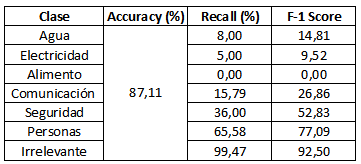
\includegraphics[scale=0.8]{images/MetricasClasificador.png}
        \caption[Métricas del clasificador.]{Métricas del clasificador.\\Fuente: Elaboración Propia, (2016)}
        \label{fig:metricasClass}
\end{figure}

Los valores expuestos anteriormente son interpretados, respectivamente, como sigue a continuación.

\begin{itemize}
\item \textit{Accuracy}: Este valor quiere decir qué con, aproximadamente, un 87\% al decir que un elemento pertenece a una determinada clase esa predicción es correcta.
\item \textit{Recall}: Este valor quiere decir que para una clase en particular, es posible identificar es posible identificar en un determinado porcentaje $p$, correspondiente al valor presentado en la Figura \ref{fig:metricasClass}, de los elementos pertenecientes a aquella clase.
\item \textit{F-1 Score}: Corresponde al \textit{trade-off} entre \textit{accuracy} y \textit{recall}, al incrementar uno, el otro disminuirá en un $F$\% descrito por los valores en la Figura \ref{fig:metricasClass}.
\end{itemize}

En particular este clasificador cuenta con alta precisión y bajo \textit{recall}, eso significa que el es preciso para clasificar, pero no es capaz de clasificar algunos de los casos particulares de cada clase. Esto se debe al conjunto de entrenamiento utilizado, los datos no están balanceados para cada clase, es decir, la clase A, no tiene los mismos elementos que la clase B, ésto repercute en que debido a las pocas instancias que tiene el algoritmo para aprender no es capaz de reconocer elementos de la clase con menos elementos. En particular el caso de la clase "Alimentos", los datos que se utilizaron son del periodo inmediato al evento, por ello no se encontraron demasiados elementos que hagan referencia a la falta de alimento en una población.

\section{Topología y replicación}
\label{sec:topYPar}

En la sección \ref{subsubsec:topologiaSistema} se explicitó cómo están dispuestos los operadores en la topología, pero se ha de recordar que el sistema está pensado para operar en casos de emergencia y ha de ser capáz de escalar de acuerdo a las necesidades de la situación.

\textit{Apache Storm} es capaz de realizar lo anterior, pero se ha de especificar el máximo número de nodos que tiene cada nivel de operadores. Para explicar lo anterior se utilizan las Figuras \ref{fig:Implementacion1} y \ref{fig:Implementacion1p2} que muestran la implementación del la topología y una esquematización de cómo se comporta en la peor situación, es decir, cuando el sistema determine que el nivel de replicación debe ser máximo.

\begin{figure}[H]
	\centering
	\captionsetup{justification=centering}
	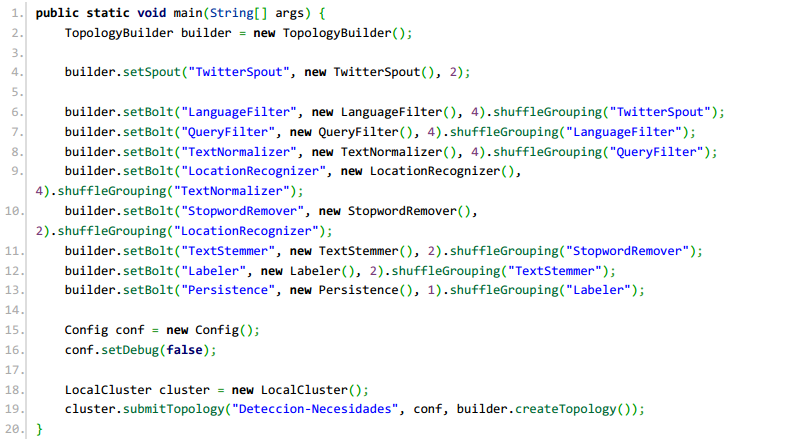
\includegraphics[scale=0.8]{images/ImplementacionTopologia1.png}
	\caption[Implementación topología de detección de necesidades.]{Implementación topología de detección de necesidades.\\Fuente: Elaboración Propia, (2016)}
	\label{fig:Implementacion1}
\end{figure}

Cada elemento de procesamiento, \textit{bolt}, es instanciado, el valor que acompaña a cada uno de ellos es el numero máximo de nodos que tiene el sistema y seguido del modo de agrupamiento, en este caso, \textit{shuffle grouping} para balancear la carga en cada nodo.

\begin{figure}[H]
	\centering
	\captionsetup{justification=centering}
	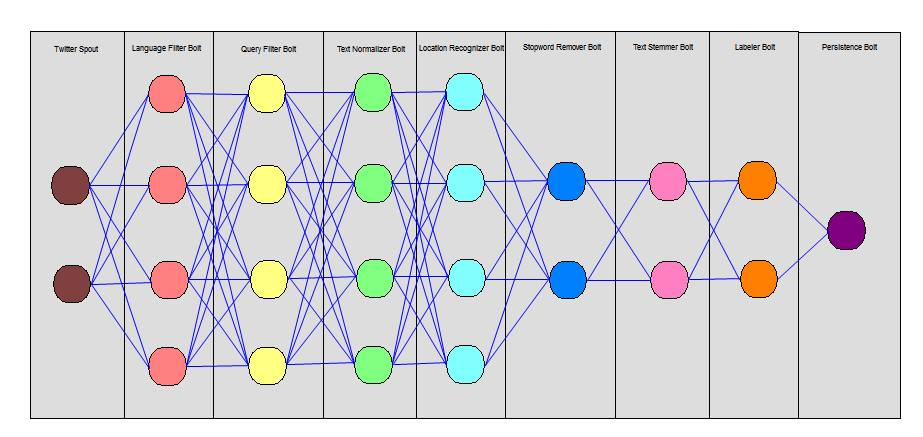
\includegraphics[scale=0.5]{images/ImplementacionTopologia1.2.png}
	\caption[Esquema de la topología en el caso de máxima actividad.]{Esquema de la topología en el caso de máxima actividad.\\Fuente: Elaboración Propia, (2016)}
	\label{fig:Implementacion1p2}
\end{figure}

Cada línea de este esquema señala comunicación de izquierda a derecha. En el caso de que el sistema trabaje al máximo de su capacidad cada nodo enviará, \textit{round robin}, estados al siguiente nivel.

Esta implementación y diagrama reflejan la solución inicial la cual fue decidida arbitrariamente para probar el sistema.

Tempranamente se detectó que el hecho de tener dos \textit{spout} resultaba contraproducente, pues enviaba, en repetidas ocaciones, el mismo estado al sistema, es decir, cuando el \textit{spout} A enviaba el estado $e_{0}$, probablemente el \textit{spout} B enviase el mismo estado $e_{0}$. Por ello se decidió eliminar el segundo \textit{spout} y limitarlo sólo a uno.

Se utilizó el tiempo de ejecución para 1000, 2000, 4000 y 8000 estados, pertenecientes al terremoto de Concepción el año 2010 para seleccionar cuán numeroso debería ser un nivel de nodos. Sus resultados son expuestos en la tabla \ref{tab:estadisticas}.

\begin{table}[H]
\centering
\caption[Estadísticas de los operadores para 1000, 2000, 4000 y 8000 estados.]{Estadísticas de los operadores para 1000, 2000, 4000 y 8000 estados.\\Fuente: Elaboración Propia, (2016)}
\label{tab:estadisticas}
\begin{tabular}{|c|c|c|c|c|c|}
\hline
\multirow{2}{*}{\textbf{\begin{tabular}[c]{@{}c@{}}Entradas \\ (estados)\end{tabular}}} & \multirow{2}{*}{\textbf{Métricas}} & \multicolumn{4}{c|}{\textbf{Operadores}} \\ \cline{3-6} 
 &  & \textbf{Idioma} & \textbf{Normalizador} & \textbf{Ubicación} & \textbf{Stopword} \\ \hline
\multirow{4}{*}{\textbf{1000}} & \textbf{Procesados} & 1000 & 1000 & 1000 & 1000 \\ \cline{2-6} 
 & \textbf{Emitidos} & 402 (40.20\%) & 1000 (100\%) & 623 (62.30\%) & 1000 (100\%) \\ \cline{2-6} 
 & \textbf{Descartados} & 598 (59.80\%) & 0 (0\%) & 377 (37.70\%) & 0 (0\%) \\ \cline{2-6} 
 & \textbf{\begin{tabular}[c]{@{}c@{}}Tiempo \\ (ms)\end{tabular}} & 0.77 & 36,45 & 2111.73 & 30.54 \\ \hline
\multirow{4}{*}{\textbf{2000}} & \textbf{Procesados} & 2000 & 2000 & 2000 & 2000 \\ \cline{2-6} 
 & \textbf{Emitidos} & 807 (40.35\%) & 2000 (100\%) & 1058 (52.90\%) & 2000 (100\%) \\ \cline{2-6} 
 & \textbf{Descartados} & 1193 (59.65\%) & 0 (0\%) & 942 (47.10\%) & 0 (0\%) \\ \cline{2-6} 
 & \textbf{\begin{tabular}[c]{@{}c@{}}Tiempo\\ (ms)\end{tabular}} & 0.84 & 56.07 & 1314.53 & 45.23 \\ \hline
\multirow{4}{*}{\textbf{4000}} & \textbf{Procesados} & 4000 & 4000 & 4000 & 4000 \\ \cline{2-6} 
 & \textbf{Emitidos} & 1673 (41.83\%) & 4000 (100\%) & 1985 (49.63\%) & 4000 (100\%) \\ \cline{2-6} 
 & \textbf{Descartados} & 2327 (58.17\%) & 0 (0\%) & 2015 (50.37\%) & 0 (0\%) \\ \cline{2-6} 
 & \textbf{\begin{tabular}[c]{@{}c@{}}Tiempo\\ (ms)\end{tabular}} & 2.08 & 49.09 & 2155.30 & 71.09 \\ \hline
\multirow{4}{*}{\textbf{8000}} & \textbf{Procesados} & 8000 & 8000 & 8000 & 8000 \\ \cline{2-6} 
 & \textbf{Emitidos} & 3101 (38.76\%) & 8000 (100\%) & 4113 (51.41\%) & 8000 (100\%) \\ \cline{2-6} 
 & \textbf{Descartados} & 4899 (61.24\%) & 0 (\%) & 3887 (48.59\%) & 0 (0\%) \\ \cline{2-6} 
 & \textbf{\begin{tabular}[c]{@{}c@{}}Tiempo\\ (ms)\end{tabular}} & 3.37 & 59.53 & 4442.00 & 87.24 \\ \hline
\end{tabular}
\end{table}

Con estos resultados se busca definir los valores para la cantidad de nodos por cada nivel de \textit{bolts}, de los resultados presentados en la Tabla \ref{tab:estadisticas} podemos concluir lo siguiente:

Para el caso del operador filtro de idioma, para diferentes tamaños de conjuntos de estados, es emitido, aproximadamente, un 40.28\% del flujo de información que llega a aquel operador. Tiene un tiempo de ejecución reducido en comparación a los demás operadores.

En operadores normalizadores de texto y eliminación de \textit{stopwords} todo estado que llega es emitido.

El operador de ubicación admite, aproximadamente, un 54.06\% y presenta un elevado tiempo de ejecución.

Estos resultados muestran el comportamiento individual de cada uno de éstos bolts, pero su operación no es de esta forma, por ello se preparó el mismo conjunto de pruebas de 1000, 2000, 4000 y 8000 datos aleatoreos del conjunto de datos del terremoto de Concepción el año 2010 y se pasó al sistema para ver la cantidad de estados emitidos en cada caso. Para el caso del operador de consulta se utilizaron los términos "terremoto", "concepción" y "Chile". Se restringió el paralelismo de la topología completa para realizar estas pruebas, es decir, cada operador tuvo, como máximo, una instancia trabajando durante todo el proceso.

\begin{table}[H]
\centering
\caption[Prueba sistema completo utilizando 1000 estados.]{Prueba sistema completo utilizando 1000 estados.\\Fuente: Elaboración Propia, (2016)}
\label{PruebaSistFull1000}
\begin{tabular}{|c|l|l|}
\hline
\textbf{Cantidad} & \multicolumn{2}{c|}{\textbf{1000}} \\ \hline
\textbf{Operador} & \multicolumn{1}{c|}{\textbf{Estados recibidos}} & \multicolumn{1}{c|}{\textbf{Estados emitidos}} \\ \hline
Spout & 1000 & 1000 \\ \hline
Idioma & 1000 & 402 \\ \hline
Consulta & 402 & 123 \\ \hline
Normalizador & 123 & 123 \\ \hline
Ubicacion & 123 & 0 \\ \hline
Stopword & 0 & 0 \\ \hline
Stemmer & 0 & 0 \\ \hline
Etiquetador & 0 & 0 \\ \hline
Persistencia & 0 & 0 \\ \hline
\end{tabular}
\end{table}

\begin{table}[H]
\centering
\caption[Prueba sistema completo utilizando 2000 estados.]{Prueba sistema completo utilizando 2000 estados.\\Fuente: Elaboración Propia, (2016)}
\label{PruebaSistFull2000}
\begin{tabular}{|c|l|l|}
\hline
\textbf{Cantidad} & \multicolumn{2}{c|}{\textbf{2000}} \\ \hline
\textbf{Operador} & \multicolumn{1}{c|}{\textbf{Estados recibidos}} & \multicolumn{1}{c|}{\textbf{Estados emitidos}} \\ \hline
Spout & 2000 & 2000 \\ \hline
Idioma & 2000 & 807 \\ \hline
Consulta & 807 & 78 \\ \hline
Normalizador & 78 & 78 \\ \hline
Ubicacion & 78 & 0 \\ \hline
Stopword & 0 & 0 \\ \hline
Stemmer & 0 & 0 \\ \hline
Etiquetador & 0 & 0 \\ \hline
Persistencia & 0 & 0 \\ \hline
\end{tabular}
\end{table}

\begin{table}[H]
\centering
\caption[Prueba sistema completo utilizando 4000 estados.]{Prueba sistema completo utilizando 4000 estados.\\Fuente: Elaboración Propia, (2016)}
\label{PruebaSistFull4000}
\begin{tabular}{|c|l|l|}
\hline
\textbf{Cantidad} & \multicolumn{2}{c|}{\textbf{4000}} \\ \hline
\textbf{Operador} & \multicolumn{1}{c|}{\textbf{Estados recibidos}} & \multicolumn{1}{c|}{\textbf{Estados emitidos}} \\ \hline
Spout & 4000 & 4000 \\ \hline
Idioma & 4000 & 1673 \\ \hline
Consulta & 1673 & 39 \\ \hline
Normalizador & 39 & 39 \\ \hline
Ubicacion & 39 & 0 \\ \hline
Stopword & 0 & 0 \\ \hline
Stemmer & 0 & 0 \\ \hline
Etiquetador & 0 & 0 \\ \hline
Persistencia & 0 & 0 \\ \hline
\end{tabular}
\end{table}

\begin{table}[H]
\centering
\caption[Prueba sistema completo utilizando 8000 estados.]{Prueba sistema completo utilizando 8000 estados.\\Fuente: Elaboración Propia, (2016)}
\label{PruebaSistFull8000}
\begin{tabular}{|c|l|l|}
\hline
\textbf{Cantidad} & \multicolumn{2}{c|}{\textbf{8000}} \\ \hline
\textbf{Operador} & \multicolumn{1}{c|}{\textbf{Estados recibidos}} & \multicolumn{1}{c|}{\textbf{Estados emitidos}} \\ \hline
Spout & 8000 & 8000 \\ \hline
Idioma & 8000 & 3101 \\ \hline
Consulta & 3101 & 151 \\ \hline
Normalizador & 151 & 151 \\ \hline
Ubicacion & 151 & 0 \\ \hline
Stopword & 0 & 0 \\ \hline
Stemmer & 0 & 0 \\ \hline
Etiquetador & 0 & 0 \\ \hline
Persistencia & 0 & 0 \\ \hline
\end{tabular}
\end{table}

Las Tablas \ref{PruebaSistFull1000}, \ref{PruebaSistFull2000}, \ref{PruebaSistFull4000} y \ref{PruebaSistFull8000} muestran respectivamente los resultados para los datos antes mencionados, estos resultados muestran la dificultad que tiene un estado para completar el proceso, pero hace presumir un error de implemenación en el operador de ubicación. Para descargar que se deba a los datos se incrementó en gran medida el número de éstos conformando los resultados entregados en la Tabla \ref{tab:PruebaSistFull30000}

\begin{table}[H]
\centering
\caption[Prueba sistema completo utilizando 30000 estados.]{Prueba sistema completo utilizando 30000 estados.\\Fuente: Elaboración Propia, (2016)}
\label{tab:PruebaSistFull30000}
\begin{tabular}{|c|l|l|}
\hline
\textbf{Cantidad} & \multicolumn{2}{c|}{\textbf{30000}} \\ \hline
\textbf{Operador} & \multicolumn{1}{c|}{\textbf{Estados recibidos}} & \multicolumn{1}{c|}{\textbf{Estados emitidos}} \\ \hline
Spout & 30000 & 30000 \\ \hline
Idioma & 30000 & 5372 \\ \hline
Consulta & 5372 & 883 \\ \hline
Normalizador & 883 & 883 \\ \hline
Ubicacion & 883 & 0 \\ \hline
Stopword & 0 & 0 \\ \hline
Stemmer & 0 & 0 \\ \hline
Etiquetador & 0 & 0 \\ \hline
Persistencia & 0 & 0 \\ \hline
\end{tabular}
\end{table}

 Ninguno de los datos contenía información sobre la ubicación, por ello el operador debe inferirla con respecto al texto, pero casos como por ejemplo el mostrado en la Tabla \ref{tab:resultadoEsperadoUbicacio} muestran que no se está realizando la labor como debiese.

 \begin{table}[H]
\centering
\caption[Resultado esperado de un estado válido para el operador ubicación.]{Resultado esperado de un estado válido para el operador ubicación.\\Fuente: Elaboración Propia, (2016)}
\label{tab:resultadoEsperadoUbicacio}
\begin{tabular}{lllll}
\cline{1-3}
\multicolumn{1}{|c|}{\textbf{Estado}} & \multicolumn{1}{c|}{\textbf{Resultado esperado}} & \multicolumn{1}{c|}{\textbf{Resultado obtenido}} &  &  \\ \cline{1-3}
\multicolumn{1}{|l|}{\begin{tabular}[c]{@{}l@{}}@tvn\_mauricio x fin internet desde el movil, \\ ciudad satelite maipu, sin luz ni agua desde \\ el terremoto casi 30 hrs\end{tabular}} & \multicolumn{1}{l|}{Emitir(-33.51667, -70.76667)} & \multicolumn{1}{l|}{No emitido} &  &  \\ \cline{1-3}
 &  &  &  &  \\
 &  &  &  & 
\end{tabular}
\end{table}

La solución a ésto fue reescribir el código del \textit{bolt} de ubicación, pues contenía un error de evaluación dentro de las condiciones para hallar la localidad contenida en el texto, además de un problema de conexión del colector de eventos para el operador de \textit{stopwords}. Habiendo corregido esto se volvió a realizar la última prueba correspondiente a la todos los estados obteniendo los resultados presentados en las Tabla \ref{tab:sistemaCompletoEstadosCorregidos}. Cabe destacar que estos datos son influenciados por el operador consulta, mientras el filtro de ubicación sólo permite el paso de elementos que hagan referencia a ubicaciones dentro del país y el filtro de idioma sólo permite el paso de aquellos que cumplan con estar en español, el filtro de consulta está influenciado en gran medida por la decisión del usuario; mientras más términos o mientras más generales éstos sean, mayor cantidad de elementos ingresa al sistema.

\begin{table}[H]
\centering
\caption[Prueba al sistema completo y corregido utilizando 30000 estados.]{Prueba al sistema completo y corregido utilizando 30000 estados.\\Fuente: Elaboración Propia, (2016)}
\label{tab:sistemaCompletoEstadosCorregidos}
\begin{tabular}{|c|l|l|}
\hline
\textbf{Cantidad} & \multicolumn{2}{c|}{\textbf{30000}} \\ \hline
\textbf{Operador} & \multicolumn{1}{c|}{\textbf{Estados recibidos}} & \multicolumn{1}{c|}{\textbf{Estados emitidos}} \\ \hline
Spout & 30000 & 30000 \\ \hline
Idioma & 30000 & 5372 \\ \hline
Consulta & 5372 & 883 \\ \hline
Normalizador & 883 & 883 \\ \hline
Ubicacion & 883 & 743 \\ \hline
Stopword & 743 & 743 \\ \hline
Stemmer & 743 & 743 \\ \hline
Etiquetador & 743 & 743 \\ \hline
Persistencia & 743 & 743 \\ \hline
\end{tabular}
\end{table}

Estos resultados distan de los realizados para los operadores individuales y muestran que el flujo de información en el sistema haciendo uso de datos reales. Teniendo en cuenta estos resultados se modifica la topología inicial presentada en la figura \ref{fig:Implementacion1p2} y pasa a utilizarse la presentada en la Tabla \ref{tab:topologiaFinal}, sus valores se basan en el porcentaje de datos capaces de pasar el operador, siendo estos representados en la Tabla \ref{tab:topologiaFinal2}.

\begin{table}[H]
\centering
\caption[Generalización del nivel máximo de replicación de la topología.]{Generalización del nivel máximo de replicación de la topología.\\Fuente: Elaboración Propia, (2016)}
\label{tab:topologiaFinal2}
\begin{tabular}{|l|c|}
\hline
\multicolumn{1}{|c|}{\textbf{Operador}} & \textbf{Nivel de replicación} \\ \hline
Spout & 1 \\ \hline
Idioma & N \\ \hline
Consulta & C = $\ceil{18\% · N}$ \\ \hline
Normalizador & $\ceil{16\% · C}$ \\ \hline
Ubicación & U = $\ceil{16\% · C}$ \\ \hline
Stopword & S = $\ceil{84.14\% · U}$ \\ \hline
Stemmer & S \\ \hline
Etiquetador & S \\ \hline
Persistencia & S \\ \hline
\end{tabular}
\end{table}
        
Donde $N$ es un valor arbitrario determinado por el desarrollador. Para determinar un nivel de replicación para el sistema se determinó $N = 10$, así el sistema se entrega como el siguiente nivel de replicación máximo en sus operadores:

\begin{table}[]
\centering
\caption[Nivel máximo de replicación de la topología.]{Nivel máximo de replicación de la topología.\\Fuente: Elaboración Propia, (2016)}
\label{tab:topologiaFinal}
\begin{tabular}{|l|c|}
\hline
\multicolumn{1}{|c|}{\textbf{Operador}} & \textbf{Nivel de replicación} \\ \hline
Spout & 1 \\ \hline
Idioma & 10 \\ \hline
Consulta & 2 \\ \hline
Normalizador & 2 \\ \hline
Ubicación & 2 \\ \hline
Stopword & 1 \\ \hline
Stemmer & 1 \\ \hline
Etiquetador & 1 \\ \hline
Persistencia & 1 \\ \hline
\end{tabular}
\end{table} 

\section{Funcionamiento en alto tráfico}
\label{sec:AltoTrafico}

La siguiente gráfica presentada en la Figura \ref{fig:graficoDeTweets} presenta el flujo de mensajes de \textit{Twitter} entre las fechas 16 de febrero y 2 de marzo del año 2010, en ella se aprecia que se produjo un \textit{peak} de \textit{tweets} al momento de producirse el evento terremoto.

\begin{figure}[H]
        \centering
        \captionsetup{justification=centering}
        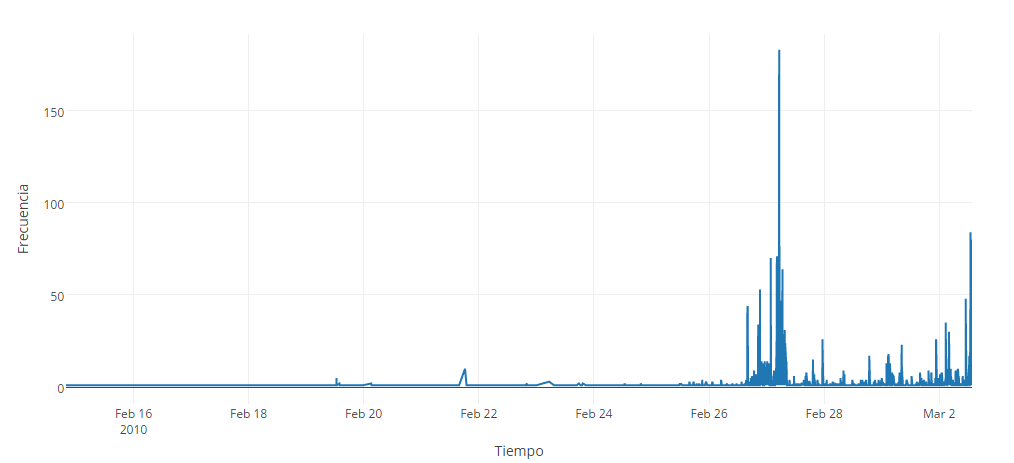
\includegraphics[scale=0.6]{images/GraficoTweetsHastaEventoZoom1.png}
        \caption[Distribución de estados presente en el conjunto de datos utilizado para evaluar.]{Distribución de estados presente en el conjunto de datos utilizado para evaluar.\\Fuente: Elaboración Propia, (2016)}
        \label{fig:graficoDeTweets}
\end{figure}

Este \textit{peak} de información sólo se ve reflejado en el sistema como en un posible aumento de los mensajes con contenido del evento, mas no una cantidad de mensajes, pues la herramienta, Twitter4J, realiza un muestreo constante. 

Teniendo en consideración lo anterior en cuanto a la cantidad de mensajes, se realizó una recopilación de eventos por un periodo de una hora del \textit{stream} actual de eventos para obtener un total de 150.800 \textit{tweets}. El gráfico presentado en la Figura \ref{fig:graficoAcumulado} presenta la cantidad eventos acumulados en función del tiempo cuya pendiente indica que se reciben 42 estados por segundo.

\begin{figure}[H]
        \centering
        \captionsetup{justification=centering}
        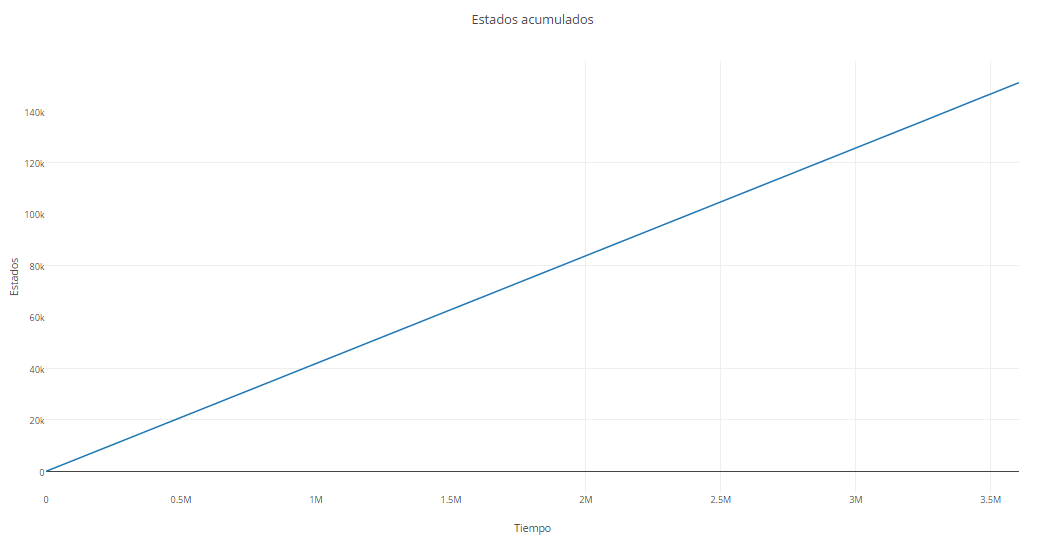
\includegraphics[scale=0.5]{images/DatosAcumulados.png}
        \caption[Recopilación de datos desde el \textit{stream}.]{Recopilación de datos desde el \textit{stream}.\\Fuente: Elaboración Propia, (2016)}
        \label{fig:graficoAcumulado}
\end{figure}

Haciendo uso de éstos resultados se simuló la llegada de los estados contenidos dentro de los datos de prueba durante una hora sobre el sistema. Los resultados de esta simulación del comportamiento de la aplicación al operar como si fuese un evento real se muestran en las Figuras \ref{}. La máquina para realizar estas pruebas fue la descrita en la sección \ref{subsec:HerrDesarrollo} y se utilizó la herramienta YourKit.


